\documentclass[10pt]{article}
\usepackage{graphicx}
\usepackage{subcaption}
\usepackage[T1]{fontenc}
\usepackage{amsmath}
\usepackage{lipsum}
\usepackage{amsfonts}
\usepackage{hyperref}
\usepackage{mathtools}
\providecommand\given{}
\usepackage[utf8]{inputenc}
\usepackage[letterpaper,margin=1in]{geometry}
\usepackage[parfill]{parskip}

\def\therefore{\boldsymbol{\text{ }
\leavevmode
\lower0.4ex\hbox{$\cdot$}
\kern-.5em\raise0.7ex\hbox{$\cdot$}
\kern-0.55em\lower0.4ex\hbox{$\cdot$}
\thinspace\text{ }}}

\vspace{-8ex}
\date{}

\graphicspath{ {./figs/} }

\begin{document}

\title{\textbf{\Large{\textsc{ECE410:} Linear Control Systems}} \\ \Large{Lab 1 Report: NL Sims?} \\ \textbf{\small{PRA101}}\vspace{-0.3cm}}
\author{Pranshu Malik, Varun Sampat \\ \footnotesize{1004138916}, \footnotesize{1003859602}\vspace{-3cm}}

\maketitle

\section{Introduction}
We have a system $G(s)$ that is very nice.


\section{Numerical integration Graphs and Evaluation (Section 3)}
This section models the system using the differential equations provided in the lab handout, and solves the DE by numerical integration. 

Recall, the given non-linear function was:
\begin{center}
   \begin{math}
    \dot{x} = f(x, t) = 
        \begin{bmatrix}
        x_2\\
        -\frac{g sin(x_1)}{l} - \frac{cos(x_1) u(t)}{ml}
        \end{bmatrix}
    \end{math} 
\end{center}

There were two initial conditions of interest:
\begin{center}
    1.
    \begin{math}
     x^0_1 = 
     \begin{bmatrix}
     0\\ \sqrt{g/l}
     \end{bmatrix}
    %  ;
    %  u^0_1 = 0
    \end{math}
\end{center}

\begin{center}
    2. 
    \begin{math}
     x^0_2 = 
     \begin{bmatrix}
     0\\1.99 \sqrt{g/l}
     \end{bmatrix}
    %  ;
    %  u^0_2 = 0
    \end{math}
\end{center}

Note, $x_1 = \theta$, and $x_2 = \dot{\theta}$. 
$\theta = 0$, but $\dot{\theta}$ is a non-zero value. This is similar to providing the pendulum with an initial velocity from its rest position (equilibrium at $\theta = 0$) at time $t = 0$.

$u(t) = 0$ for this section, implying the system behaves naturally; there is no forced response.

\subsection{Graphs for initial condition 1}
    
    \begin{figure}[h]
     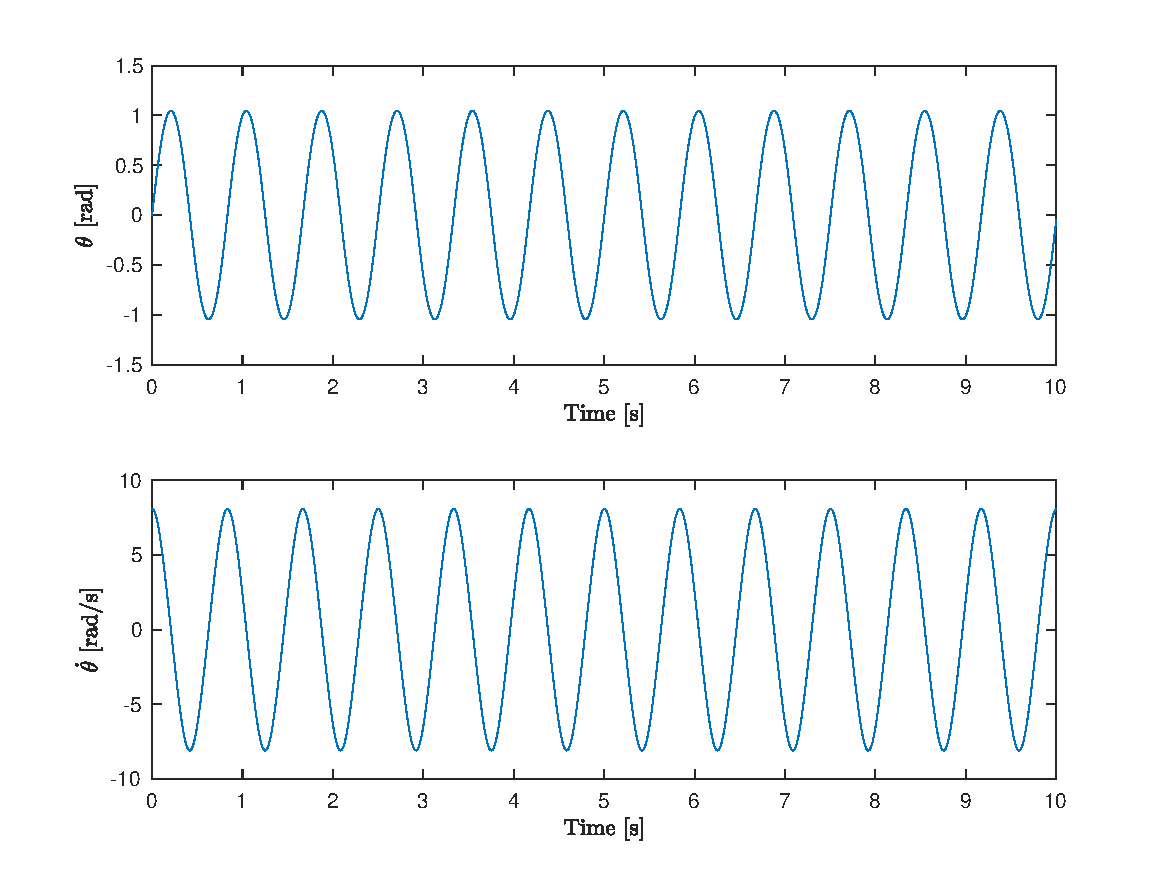
\includegraphics[scale=0.7]{lab1/figs/section3_x0_1_state_evolution.pdf}
     \caption{State Evolution to initial condition 1}
     \label{figure:x_0_1_state_evolution}
    \end{figure}
    
    \begin{figure}[ht]
     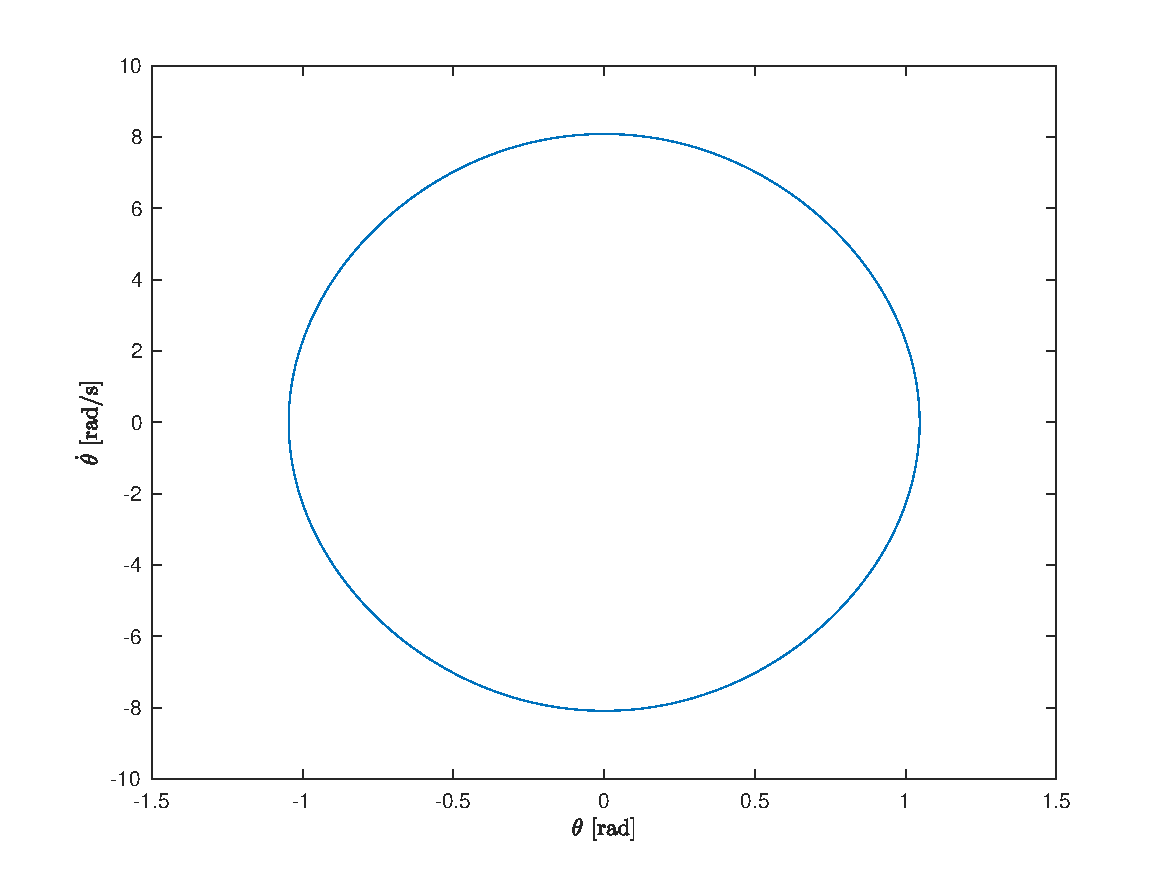
\includegraphics[scale=0.7]{lab1/figs/section3_x0_1_state_orbit.pdf}
     \caption{State orbit for initial condition 1}
     \label{figure:x_0_1_state_evolution}
    \end{figure}

\subsection{Graphs for initial condition 2}
    \begin{figure}[ht]
     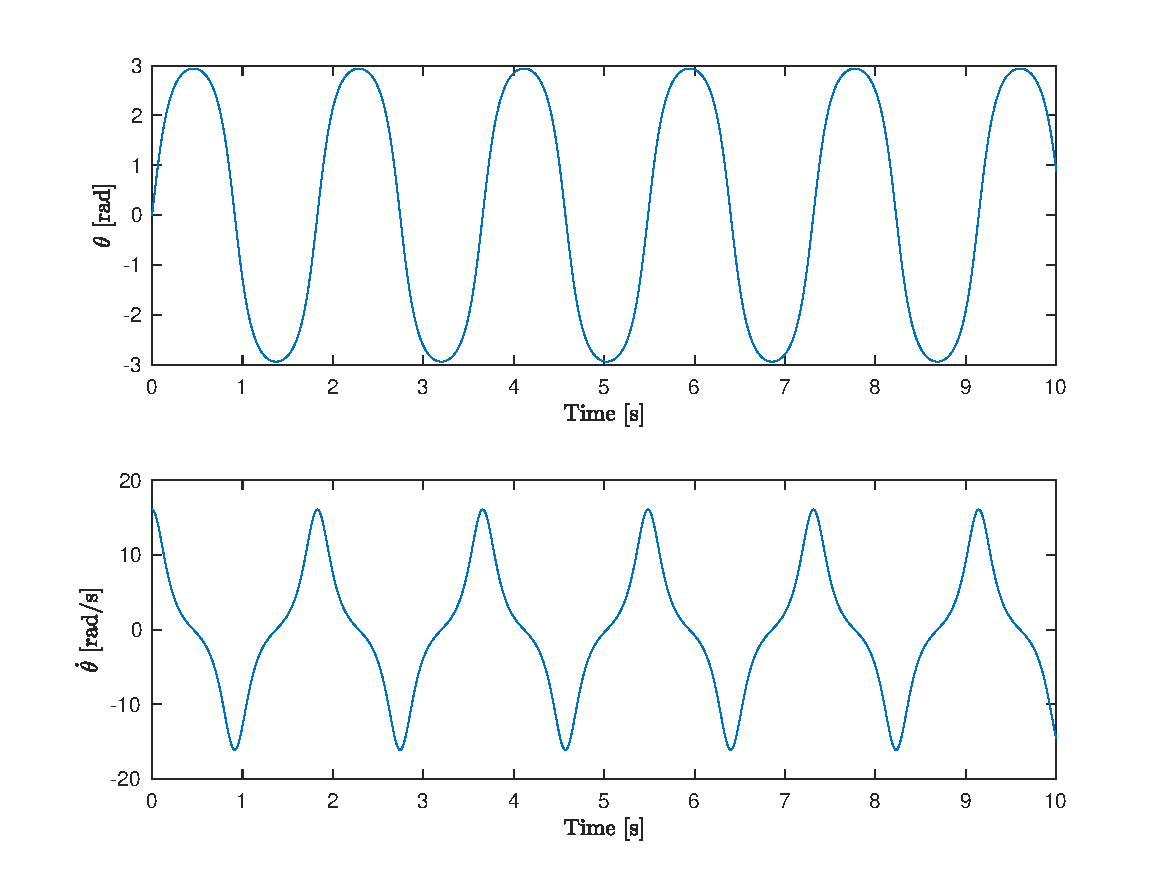
\includegraphics[scale=0.7]{lab1/figs/section3_x0_2_state_evolution.pdf}
     \caption{State Evolution to initial condition 2}
     \label{figure:x_0_2_state_evolution}
    \end{figure}

    \begin{figure}[ht]
     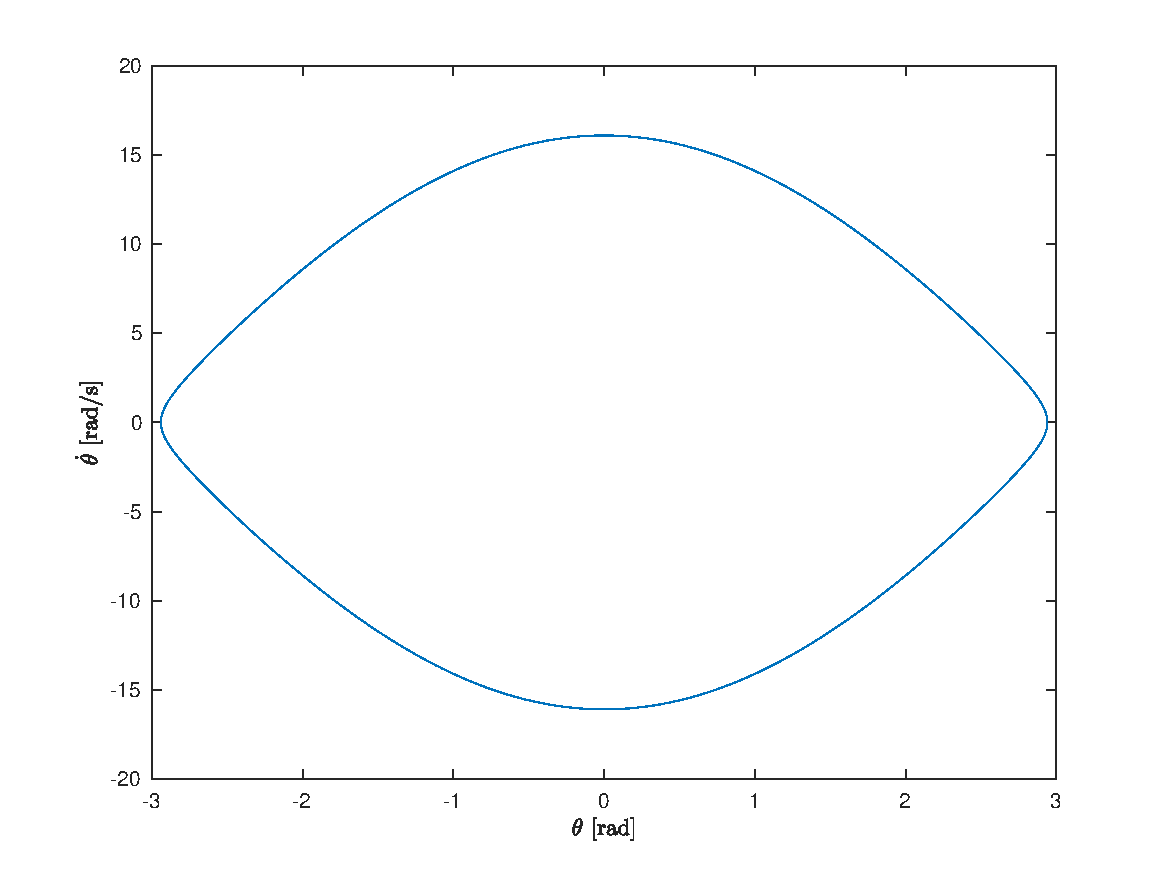
\includegraphics[scale=0.7]{lab1/figs/section3_x0_2_state_orbit.pdf}
     \caption{State orbit for initial condition 2}
     \label{figure:x_0_1_state_orbit}
    \end{figure}

\subsection{Comparison/Analysis}
    For the first initial condition, the system response is clearly sinusoidal. For the second initial condition, however, the response is not sinusoidal. The frequency of the first initial condition is higher than the frequency of the second initial condition, on visual introspection. 
    
    To understand the difference in the responses, it is important to identify what distinguishes the initial conditions. The first condition basically injects a lower angular velocity (and hence, a lower linear velocity) than the second initial condition. Since no energy is lost here, the pendulum should sweep a higher angle for a higher initial velocity. This is seen in figures 2 and 4, where the \begin{math}
     max(\theta)_1 << max(\theta)_2
    \end{math}.
    
    Because initial condition 2 reaches a higher value of $\theta$ ($\sim$ 3 radians), one would expect a higher time period and hence a lower frequency than initial condition 1, that only goes up to $\sim$ 1 radian. 
    
    3 radians is $\sim$ $\pi$ which is 180 deg, which means physically speaking, the pendulum almost reaches the top. While the shape of the graph is not 
    

\section{Symbolic Linearization (Section 4)}

\subsection{Equilibrium 1}
\begin{center}
    1.
    \begin{math}
     \dot{\Bar{x}} = 
     \begin{bmatrix}
     0\\ 0
     \end{bmatrix}
     ;
     \dot{\Bar{u}} = 0
    \end{math}
\end{center}

\subsection{Equilibrium 2}
\begin{center}
    1.
    \begin{math}
     \dot{\Bar{x}} = 
     \begin{bmatrix}
     \Bar{\theta} \\ 0
     \end{bmatrix}
     ;
     \dot{\Bar{x}} = -mg tan(\Bar{\theta})
    \end{math}
\end{center}


\section{Comparing Symbolic Linearization to Numerical Integration (Section 5)}

\end{document}
